% !TeX root = main.tex
\section{Eternity II}
	\subsection{Les origines}
		
	Eternity II est le fier successeur d'Eternity.
	
	La première version sortie en 1999, était composée de 159 pièces de différentes formes, cependant ces formes peuvent être décomposés en forme de triangles équilatéraux (ou leur moitié) qui doivent être placés sur un plateau octogonal. 
	
	\begin{figure}[H]
		\minipage{0.65\textwidth}
		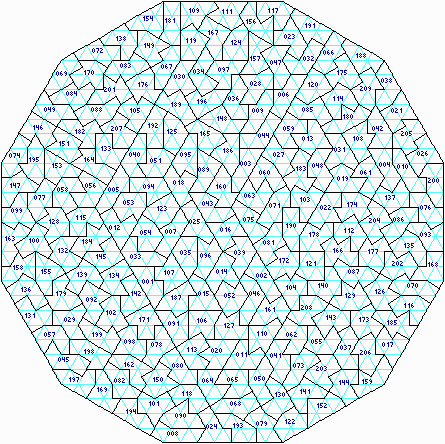
\includegraphics[width=\linewidth]{images/eternity_1.jpg}
		\caption{Eternity I}\label{fig:eternity_1}
		\endminipage\hfill
		\minipage{0.33\textwidth}
		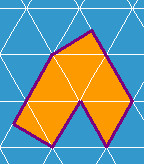
\includegraphics[width=\linewidth]{images/eternity_1_piece.jpg}
		\caption{Forme d'une pièce d'Eternity I} \label{fig:eternity_1_piece}
		\endminipage\hfill
	\end{figure}

	Son point faible se trouvait dans la disposition de ses pièces sur le plateau : il était possible de pré-calculer des régions, puis de remplir l'espace restant en s'assurant que celui-ci possède une forme adaptée aux pièces restantes \cite{resolutioneternity}.
	De cette façon, le puzzle fut résolu en à peine un an (contrairement aux 3 ans prévus par le créateur), par deux mathématiciens, qui ont ainsi empoché la récompense s'élevant à $1000000$\pounds.
	
	Après cet \enquote{échec}, Christopher Monckton, le créateur d'Eternity \cite{eternity2maker}, décide en 2008 de sortir une deuxième version, bien plus complexe, avec à la clé $2000000$\textdollar pour celui qui arriverait à la résoudre au bout de deux ans.
	
	\begin{figure}[H]
		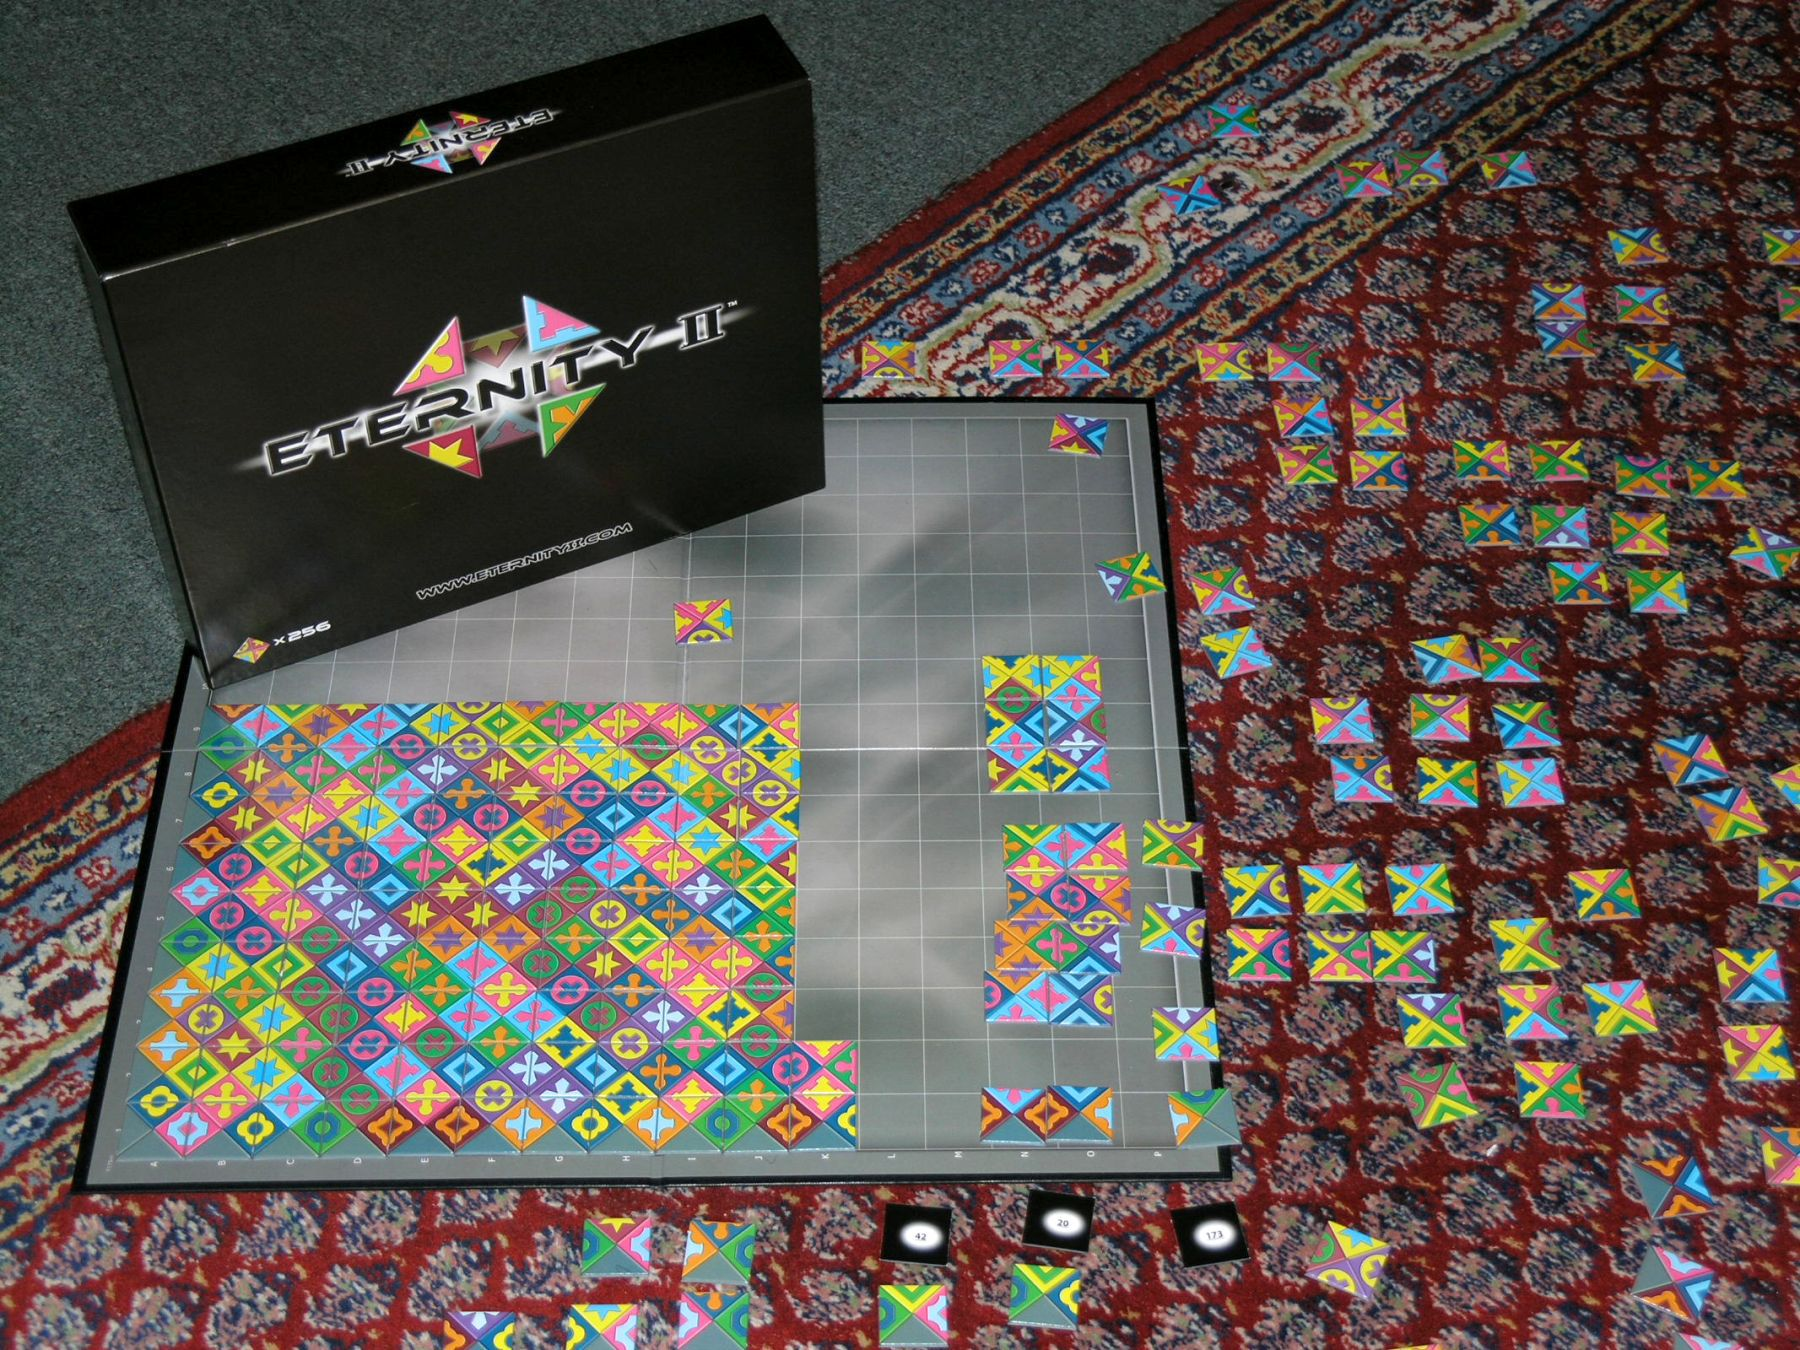
\includegraphics[width=\linewidth]{images/eternity_2.jpg}
		\caption{La boite et les pièces d'Eternity II}
		\label{fig:eternity_2}
	\end{figure}
	
	C'est un puzzle de 16 par 16 qui sort sous le nom d'Eternity II. Ce puzzle est composé de 256 pièces carrées, qui ont chacune 4 faces colorées (ou demi-motifs).
	
	Ces pièces peuvent être classées en trois catégories suivant le nombre de faces grises qu'elles possèdent :
	
	\begin{figure}[H]
	   	\minipage{0.32\textwidth}
	   	
\includegraphics[width=\linewidth]{images/piece_coin.png}
	   	\caption{\textbf{pièce de coin :} 2 faces grises}\label{fig:piece_coin}
	   	\endminipage\hfill
	   	\minipage{0.32\textwidth}
	   	
\includegraphics[width=\linewidth]{images/piece_bord.png}
	   	\caption{\textbf{pièce de bord :} 1 faces grise}\label{fig:piece_bord}
	   	\endminipage\hfill
	   	\minipage{0.32\textwidth}
	   	
\includegraphics[width=\linewidth]{images/piece_interieure.png}
	   	\caption{\textbf{pièce d'intérieur :} toutes les faces de couleur}\label{fig:piece_interieure}
	   	\endminipage
	\end{figure}

	Ces pièces ne possèdent pas de formes comme dans un puzzle classique. Afin de les faire correspondre les unes avec les autres, il est nécessaire que les faces adjacentes de chaque pièce voisine soient de la même couleur, dés lors les pièces \enquote{matchent [\autoref{fig:matching}]} .
	
	\begin{figure}[H]
		\centering
		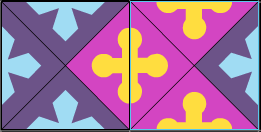
\includegraphics{images/matching_pieces.png}
		\caption{Deux pièces correctement placés (matchés)}\label{fig:matching}
	\end{figure}
	
	Par conséquent, une pièce peut quasiment être placée n'importe où sur le plateau car son placement dépend des couleurs des pièces adjacentes. De plus, les pièces n'ont pas d'orientation prédéterminée (elles peuvent être placées à n'importe quelle rotation).
	
	Pour résumer, la plupart des pièces peuvent être posées n'importe où sur le plateau à différentes rotation car la position dépends entièrement des pièces adjacentes posées auparavant. 
	
	Enfin, comme leur nom l'indique, les pièces de coins sont les seules à pouvoir être posées dans les coins du plateau, c'est aussi valable pour les pièces de bord qui ne peuvent être placées que sur les bords du plateau, ces deux types de pièces ne peuvent pas être ailleurs car leurs faces grises doivent \enquote{matcher [\autoref{fig:matching}]} avec les bords du plateau.
	
	\newpage
	\subsection{Le défi}
	
	Malgré le fait que la récompense ait expiré le 31 décembre de l'année 2010, le problème et l'enthousiasme qu'a engendré Eternity II ne s'est pas calmé pour autant (enfin si\dots un peu). Car loin d'être juste un jeu avec une importante cagnotte il recel en son c\oe ur des secrets d'une certaine valeur.
	
	En effet, jusqu'à maintenant, personne n'a réussi à résoudre ce puzzle, même pas effleuré la solution, malgré l'aide de supercalculateurs et de nombreux spécialistes, que ce soit des mathématiciens ou des informaticiens.
	
	Pourquoi ? Car derrière ce jeu anodin se cache l'un des plus grand problème du monde actuel : les problèmes NP-complets \autocite{wiki:np_complet}. Ceux-ci sont fait de telle sorte que même en connaissant leur structure ou fonctionnement, il est pratiquement impossible d'en déduire un algorithme (moyen de résoudre) efficace afin de trouver la solution. Ce type de problème est communément appliqué dans le chiffrement. Le meilleur moyen de cacher une aiguille (solution) est de la placer dans gros paquet d'aiguilles, plus le tas est gros, plus on met de temps à la [l'aiguille] trouver.
	
	\begin{exmp}
		Le nombre de combinaisons possibles pour Eternity II s'élève à $10^{545}$, c'est à dire environ $10^{450}$ fois le nombre d'atomes dans l'univers connu (estimé à au plus $10^{80}$) !!! Ca fait un gros tas d'aiguilles !!
	\end{exmp}
	
	\subsection{Les II lois d'Eternity II}
	
	Pour rendre Eternity II complexe et combinatoire, il est nécessaire de respecter les deux lois d'Eternity II :
	
	\begin{law}
		\textbf{Chaque pièce est unique}
		
		L'unicité des pièces est indispensable pour complexifier le problème, car sinon, on peux considérer qu'une pièce peux être placée à plusieurs endroits en fonction du nombre de \enquote{clones} qu'elle possède. Ce qui réduit grandement l'espace de recherche [de la solution].
	\end{law}

	\begin{law}
		\textbf{La quantité de couleurs et de pièces est finement calculée}
		
		En effet, si l'on augmente le nombre de couleurs, on obtient des couplage uniques : une pièce ne peux être couplée qu'avec une autre pièce (ou dans le meilleur des cas limite le couplage des pièces). A l'inverse, si il n'y a pas assez de couleurs, on obtient des doublons, les pièces ne sont plus uniques, ce qui va à l'encontre de la première loi.
		
		Par ailleurs, certaines couleurs sont exclusives aux pièces de coin et de bord, car ceux-ci étant liés en eux mais seulement sur le périmètre extérieur du plateau il est nécessaire d'ajouter des couleurs supplémentaires tenant compte qu'ils n'ont que 2 ou 3 faces disponibles (le reste étant des faces grises).
	\end{law}
	\newpage
	
	\subsection{État de l'art}
	
	Un grand nombre de méthodes ont été mis en place afin de résoudre ce problème.
	
	Il serait trop long de présenter et décrire les différentes méthodes mise en place car il requièrent une certaine connaissance dans les domaines auxquels ils sont appliqués. Malgré tout, les différentes approches seront notés ici à titre informatif.
	
	Pour commencer, il existe plusieurs solveurs graphiques afin de pouvoir résoudre le puzzle manuellement ou assisté par l'ordinateur. Certains d'entre eux permettent même l'import export de la progression actuelle.
	
	\begin{itemize}
		\item E2\_manual : \url{https://sourceforge.net/projects/e2manual/}(anglais)
		\item E2Lab : \url{http://eternityii.free.fr/}(anglais)
	\end{itemize}
	
	Ensuite, il existe un très grand nombre de solveurs bruteforce plus au moins rapides. Certains d'entre eux peuvent agréger plusieurs machines afin d'augmenter la puissance de calcul via le réseau.
	
	Ce problème a été abordé de façon très varié au niveau théorique et applicatif.
	
	Par exemple, Eternity à été adopté sous forme de graphe \cite{patey2010eternity} ou de sous forme de contraintes \cite{benoist2008programmation}.
	
	On note aussi un procédé intéressant de résolution grâce à une approche nommée \textbf{SAT} (satisfaisabilité booléenne) s'appuyant sur la logique propositionnelle \cite{cuvillierresolution} \cite{heule2009solving}.